\section{Posets, stores, and determinism}\label{s:lvars-lattices}

As a minimal substrate for LVars, \either{I}{we} introduce $\lambdaLVar$, a
parallel call-by-value $\lambda$-calculus extended with a \emph{store}
and with communication primitives @put@ and @get@ that operate on data
in the store.  The class of programs that \either{I am}{we are} interested in modeling
with $\lambdaLVar$ are those with explicit effectful operations on
shared data structures, in which parallel subcomputations may
communicate with each other via the @put@ and @get@ operations.

In $\lambdaLVar$, stores contain LVars.  Whereas IVars are
single-assignment variables---either empty or filled with an immutable
value---an LVar may have an arbitrary number of states forming a set
$D$, which is partially ordered by a relation $\userleq$.  An LVar can
take on any sequence of states from $D$, so long as that sequence
respects the partial order---that is, so long as updates to the LVar
(made via the @put@ operation) are \emph{inflationary} with respect to
$\userleq$.  Moreover, the @get@ operation allows only limited
observations of the LVar's state.  In this section, \either{I}{we}
discuss how posets and stores work in $\lambdaLVar$ and explain how
the semantics of @put@ and @get@ together enforce determinism in
$\lambdaLVar$ programs.

\subsection{Posets}\label{subsection:lvars-lattices}

The definition of $\lambdaLVar$ is parameterized by $D$: to write
concrete $\lambdaLVar$ programs, we must specify the set of LVar
states that we are interested in working with, and an ordering on
those states.  Therefore $\lambdaLVar$ is actually a \emph{family} of
languages, rather than a single language.

Formally, $D$ is a \emph{bounded partially ordered set}.  That is, $D$ has the following
structure:
\begin{itemize}
\item $D$ has a least element $\bot$, representing the initial
  ``empty'' state of an LVar.
\item $D$ has a greatest element $\top$, representing the ``error''
  state that results from conflicting updates to an LVar.
\item $D$ comes equipped with a partial order $\userleq$, where $\bot
  \userleq d \userleq \top$ for all $d \in D$.
\end{itemize}
We can specify all these components as a 4-tuple $(D, \userleq, \bot,
\top)$ where $D$ is a set, $\userleq$ is a partial order on the
elements of $D$, $\bot$ is the least element of $D$ according to
$\userleq$, and $\top$ is the greatest element.  However,
\either{I}{we} use $D$ as a shorthand for the entire 4-tuple $(D,
\userleq, \bot, \top)$ when its meaning is clear from the context.
\ifdefined\JOURNAL
For brevity, we say ``poset'' in place of ``bounded poset'' throughout
this paper.
\fi

Virtually any data structure to which information is added gradually
can be represented as a poset, including pairs, arrays, trees, maps,
and infinite streams.  The simplest example of a useful $D$ is one
that represents the states that a single-assignment variable (that is,
an IVar) can take on.  The states of a natural-number-valued IVar, for
instance, are the elements of the poset in
Figure~\ref{f:lvars-example-lattices}(b), that is,

\vspace{-8mm}
\singlespacing
\begin{displaymath}
  D = (\lbrace \top, \bot \rbrace \cup \mathbb{N}, \userleq, \bot, \top), 
\end{displaymath}
\doublespacing
%
where the partial order $\userleq$ is defined by setting $\bot
\userleq d \userleq \top$ and $d \userleq d$ for all $d \in D$.  This
is a poset of height three and infinite width, where the naturals
are arranged horizontally.  After the initial write of some $n \in
\mathbb{N}$, any further conflicting writes would push the state of
the IVar to $\top$ (an error).  For instance, if one thread writes $2$
and another writes $1$ to an IVar (in arbitrary order), the second of
the two writes would result in an error because $2 \sqcup 1 = \top$.

On the other hand, if we have an LVar whose states form the poset of
Figure~\ref{f:lvars-example-lattices}(a), and if we define @put@ as
least upper bound, the $\top$ state is unreachable unless we
explicitly write $\top$ to the LVar, because the lub of any two writes
is just the maximum of the two.  If one thread writes $2$ and another
writes $1$, the resulting state will be $2$, since $2 \sqcup 1 = 2$.

\ifdefined\DISSERTATION
\begin{wrapfigure}{r}{2.3in}
  \vspace{-2em}
  \begin{center}
    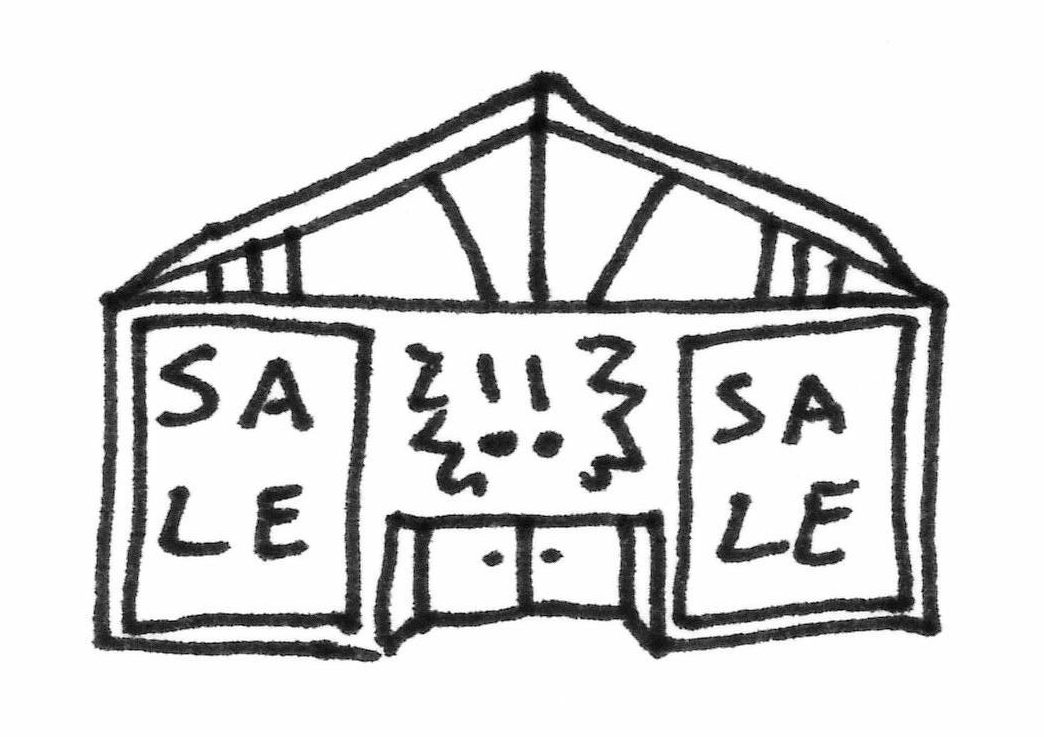
\includegraphics[scale=0.15]{../illustrations/store}
  \end{center}
  \vspace{-2em}
\end{wrapfigure}
\fi

\subsection{Inflationary, commutative updates}\label{subsection:lvars-inflationary-commutative}

For a given lattice $(D, \userleq, \bot, \top)$, we can define a set
of \emph{update operations} that determine how LVars can be updated:

\DefSetOfUpdateOperations
%
The first of the conditions in
Definition~\ref{def:set-of-update-operations} says that each update
operation is inflationary with respect to $\userleq$.  The second
condition says that update operations commute with each other.

\lk{``update'' used to be called ``bump'', but I think ``update'' is a
  better name: ``bump'' sounds like something that is
  specifically \emph{not} idempotent, while ``update'' is merely
  something that \emph{doesn't have to be} idempotent.}

In Section~\ref{s:lvars-examples}, we said that the @put@ operation on
LVars computes a least upper bound.  We can formulate the lub
operation as a set of update operations where each $u_i$ returns the
lub of its argument and some element of $D$.  This set of update
operations meets the above two conditions, but in general, update
operations need not compute a lub.  The definition of the
$\lambdaLVar$ language must be parameterized not only by the lattice
$D$, but also by the set of update operations $U$, and we will write
$\PUTi$ to denote the the @put@ operation that corresponds to update
operation $u_i$.  Since lub updates are a common and useful special
case, we will continue to write @put@ with no subscript (and with an
additional argument, as in $\putexp{\mathit{lv}}{3}$) to denote
least-upper-bound update operations.

It is important to keep in mind that least-upper-bound @put@
operations do not necessarily mix with arbitrary $\PUTi$ operations on
the same LVar.  For example, consider a family of update operations
$\{ u_{(+1)}, u_{(+2)}, \dots \}$ for atomically incrementing a
counter represented by a natural number LVar, with a lattice ordered
by the usual ordering $\leq$ on natural numbers.  The $u_{(+1)}$
operation increments the counter by one, $u_{(+2)}$ increments it by
two, and so on.  It is easy to see that these operations commute.
However, a @put@ of $4$ and a $u_{(+1)}$ do not commute: if we start
with an initial state of $0$ and the @put@ occurs first, then the
state of the LVar changes to $4$ since $\max(0, 4) = 4$, and the
subsequent $u_{(+1)}$ updates it to $5$.  But if the $u_{(+1)}$
happens first, then the final state of the LVar will be $\max(1, 4) =
4$.

In practice, the author of a particular LVar data structure must
choose which update operations that data structure should provide, and
it is the data structure author's responsibility to ensure that they
commute.  For example, the LVish Haskell library of
\either{Chapter}{Section}~\ref{ch:lvish} provides a set data
structure, @Data.LVar.Set@, that supports only @put@, whereas the
counter data structure @Data.LVar.Counter@ supports only increment
operations; an attempt to call @put@ on a @Counter@ would be ruled out
by the type system.  However, \emph{composing} LVars that support
different families of update operations is fine.  For example, an LVar
could represent a monotonically growing set (that supports @put@) of
counter LVars, where each counter is itself monotonically increasing
and supports only increment operations.  Indeed, the PhyBin case study
that \either{I}{we} describe in Section~\ref{s:lvish-phybin} uses just
such a collection of counters.

\subsection{Stores}\label{subsection:lvars-stores}

During the evaluation of a $\lambdaLVar$ program, a \emph{store} $S$
keeps track of the states of LVars.  Each LVar is represented by a
\emph{binding} that maps a location $l$, drawn from a countably infinite
set $\Loc$, to a \emph{state}, which is some element $d \in D$.
Although each LVar in a program has its own state, the states of all
the LVars are drawn from the same lattice $D$.\footnote{In practice,
  different LVars in a program might correspond to different lattices (and,
  in the LVish Haskell library that \either{I}{we} will present in
  \either{Chapter}{Section}~\ref{ch:lvish}, they do).  Multiple lattices can in
  principle be encoded using a sum construction, so this modeling
  choice is just to keep the presentation simple.}

\LVarsDefStore
%
\either{I}{We} use the notation $\extSRaw{S}{l}{d}$ to denote
extending $S$ with a binding from $l$ to $d$.  If $l \in \dom{S}$,
then $\extSRaw{S}{l}{d}$ denotes an update to the existing binding for
$l$, rather than an extension.  Another way to denote a store is by
explicitly writing out all its bindings, using the notation
$\store{\storebindingRaw{l_1}{d_1}, \dots,
  \storebindingRaw{l_n}{d_n}}$.  A store cannot contain a binding
$\storebindingRaw{l}{\top}$, because (as we will see shortly) any
write that would take the state of some location $l$ to $\top$ would
raise an error before the write can occur.

\subsection{Communication primitives}\label{subsection:lvars-communication-primitives}

The @new@, $\PUTi$, and @get@ operations create, write to, and read
from LVars, respectively. The interface is similar to that presented
by mutable references:

\begin{itemize}
\item @new@ extends the store with a binding for a new LVar whose
  initial state is $\bot$, and returns the location $l$ of that LVar
  (\ie, a pointer to the LVar).
\item $\PUTi$ takes a pointer to an LVar and updates the LVar's state
  according to the update operation $u_i \in U$, potentially pushing the
  state of the LVar upward in the lattice.  Any update that would take
  the state of an LVar to $\top$ results in an error.
\item @get@ performs a blocking ``threshold'' read that allows limited
  observations of the state of an LVar.  It takes a pointer to an LVar
  and a \emph{threshold set} $T$, which is a non-empty subset of $D$
  that is \emph{pairwise incompatible}, meaning that the lub of any
  two distinct elements in $T$ is $\top$.  If the LVar's state $d_1$
  in the lattice is \emph{at or above} some $d_2 \in T$, the @get@
  operation unblocks and returns $d_2$.  Note that $d_2$ is a unique
  element of $T$, for if there is another $d_2' \neq d_2$ in the
  threshold set such that $d_2' \userleq d_1$, it would follow that
  $d_2 \sqcup d_2' \userleq d_1$, and so $d_2 \sqcup d_2'$ cannot be
  $\top$, which contradicts the requirement that $T$ be pairwise
  incompatible.
\end{itemize}
%
The intuition behind @get@ is that it specifies a subset of the
lattice that is ``horizontal'': no two elements in the threshold set
can be above or below one another.  Intuitively, each element in the
threshold set is an ``alarm'' that detects the activation of itself or
any state above it.  One way of visualizing the threshold set for a
@get@ operation is as a subset of edges in the lattice that, if
crossed, set off the corresponding alarm.  Together these edges form a
``tripwire''.  Figure~\ref{f:lvars-example-lattices}(c) shows what the
``tripwire'' looks like for an example @get@ operation.  The
threshold set $\stateset{(\bot, 0), (\bot, 1), ...}$ (or a subset
thereof) would pass the incompatibility test, as would the threshold
set $\stateset{(0, \bot), (1, \bot), ...}$ (or a subset thereof), but
a combination of the two would not pass.

The requirement that the elements of a threshold set be pairwise
incompatible limits the expressivity of threshold sets.  In fact, it
is a stronger requirement than we need to ensure determinism.  Later
on, in Section~\ref{s:lvars-generalizing}, \either{I}{we} will explain how to
generalize the definition of threshold sets to allow more programs
to be expressed.  For now, \either{I}{we} will proceed with the simpler definition
above.
